\documentclass[aspectratio=169,11pt]{beamer}

% ============================ theme & packages ============================
\usetheme{Boadilla}
\usecolortheme{seahorse}
\setbeamertemplate{navigation symbols}{}
\setbeamertemplate{itemize item}{\textbullet}
\setbeamertemplate{blocks}[rounded][shadow=false]

\usepackage[T1]{fontenc}
\usepackage[utf8]{inputenc}
\usepackage{lmodern}
\usepackage{amsmath,amssymb,bm}
\usepackage{xcolor}
\usepackage{tikz}
\usetikzlibrary{arrows.meta,positioning}

% ----- palette (matches docs/compositional_vae_slides.tex) -----
\definecolor{cSimplex}{HTML}{2563EB}  % PhILR   (blue)
\definecolor{cLik}{HTML}{C2410C}      % TreeDTM (orange)
\definecolor{cLatent}{HTML}{7C3AED}   % CAPDA   (purple)
\definecolor{cAccent}{HTML}{BE185D}
\definecolor{cMuted}{HTML}{475569}

\newcommand{\ilr}{\operatorname{ilr}}
\newcommand{\clr}{\operatorname{clr}}

\tikzset{
  arrow/.style={-{Latex[length=1.6mm]}, semithick, draw=cMuted},
  leaf/.style ={draw, circle, inner sep=0pt, minimum size=3.2mm, fill=cLik!16, draw=cLik},
  inode/.style={draw, circle, inner sep=0pt, minimum size=3.2mm, fill=cLik!35, draw=cLik},
}

% tighter, calmer bullet lists inside the cards
\setbeamertemplate{itemize/enumerate body begin}{\scriptsize}

% uniform card body height so all three cards align to a shared baseline
\newcommand{\cardbodyH}{3.6cm}

\begin{document}

\begin{frame}{Three compositional, tree-aware VAEs --- at a glance}

  \begin{columns}[T]

  % ----------------------------- PhILR-VAE -----------------------------
  \begin{column}{0.32\textwidth}
    {\setbeamercolor{block title}{fg=white,bg=cSimplex}%
     \setbeamercolor{block body}{bg=cSimplex!7}%
    \begin{block}{\centering PhILR-VAE}
      \begin{minipage}[t][\cardbodyH][t]{\linewidth}
      \centering
      \begin{minipage}[c][1.3cm][c]{\linewidth}\centering
      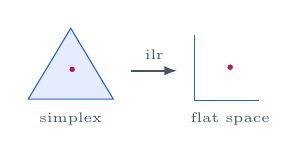
\begin{tikzpicture}[scale=0.9]
        \fill[cSimplex!12,draw=cSimplex] (0,0)--(1.2,0)--(0.6,1.0)--cycle;
        \fill[cAccent] (0.62,0.42) circle (1.1pt);
        \node[font=\tiny,cMuted] at (0.6,-0.28){simplex};
        \draw[arrow] (1.45,0.4)--(2.1,0.4);
        \node[font=\tiny,cMuted] at (1.78,0.62){$\ilr$};
        \draw[cSimplex] (2.35,-0.02)--(2.35,0.9); \draw[cSimplex] (2.35,-0.02)--(3.25,-0.02);
        \fill[cAccent] (2.85,0.45) circle (1.1pt);
        \node[font=\tiny,cMuted] at (2.85,-0.28){flat space};
      \end{tikzpicture}
      \end{minipage}
      \par\smallskip
      \raggedright\footnotesize
      \emph{Make the geometry flat, then use a vanilla VAE.}
      \begin{itemize}\setlength\itemsep{3pt}
        \item \textbf{Tree} $\to$ an orthonormal \emph{balance basis} $\Psi$.
        \item \textbf{Recon:} logistic-normal --- exact, no extra penalty.
      \end{itemize}
      \end{minipage}
    \end{block}}
  \end{column}

  % ----------------------------- TreeDTM-VAE ---------------------------
  \begin{column}{0.32\textwidth}
    {\setbeamercolor{block title}{fg=white,bg=cLik}%
     \setbeamercolor{block body}{bg=cLik!7}%
    \begin{block}{\centering TreeDTM-VAE}
      \begin{minipage}[t][\cardbodyH][t]{\linewidth}
      \centering
      \begin{minipage}[c][1.3cm][c]{\linewidth}\centering
      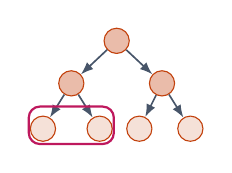
\begin{tikzpicture}[scale=0.72]
        \node[inode] (r) at (1.5,1.2){};
        \node[inode] (a) at (0.7,0.45){};
        \node[inode] (b) at (2.3,0.45){};
        \node[leaf] (l1) at (0.2,-0.35){};
        \node[leaf] (l2) at (1.2,-0.35){};
        \node[leaf] (l3) at (1.9,-0.35){};
        \node[leaf] (l4) at (2.8,-0.35){};
        \draw[arrow](r)--(a); \draw[arrow](r)--(b);
        \draw[arrow](a)--(l1); \draw[arrow](a)--(l2);
        \draw[arrow](b)--(l3); \draw[arrow](b)--(l4);
        \draw[cAccent,thick,rounded corners] (-0.05,-0.62) rectangle (1.45,0.04);
      \end{tikzpicture}
      \end{minipage}
      \par\smallskip
      \raggedright\footnotesize
      \emph{Put a likelihood at every node of the tree.}
      \begin{itemize}\setlength\itemsep{3pt}
        \item \textbf{Tree} $\to$ one local \emph{split} per internal node.
        \item \textbf{Recon:} per-clade Dirichlet-tree-multinomial.
      \end{itemize}
      \end{minipage}
    \end{block}}
  \end{column}

  % ----------------------------- CAPDA-VAE -----------------------------
  \begin{column}{0.32\textwidth}
    {\setbeamercolor{block title}{fg=white,bg=cLatent}%
     \setbeamercolor{block body}{bg=cLatent!7}%
    \begin{block}{\centering CAPDA-VAE}
      \begin{minipage}[t][\cardbodyH][t]{\linewidth}
      \centering
      \begin{minipage}[c][1.3cm][c]{\linewidth}\centering
      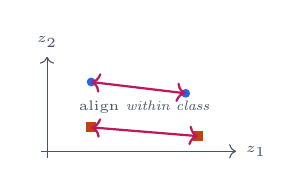
\begin{tikzpicture}[scale=0.8]
        \draw[->,cMuted] (-0.1,0)--(3.0,0); \draw[->,cMuted] (0,-0.1)--(0,1.5);
        \node[font=\tiny,cMuted,right] at (3.0,0){$z_1$};
        \node[font=\tiny,cMuted,above] at (0,1.5){$z_2$};
        \fill[cSimplex] (0.7,1.1) circle (2pt);
        \fill[cSimplex] (2.2,0.92) circle (2pt);
        \draw[<->,cAccent,thick] (0.7,1.1)--(2.2,0.92);
        \fill[cLik] (0.62,0.30) rectangle (0.78,0.46);
        \fill[cLik] (2.32,0.16) rectangle (2.48,0.32);
        \draw[<->,cAccent,thick] (0.7,0.38)--(2.4,0.24);
        \node[font=\tiny,cMuted] at (1.55,0.70){align \emph{within class}};
      \end{tikzpicture}
      \end{minipage}
      \par\smallskip
      \raggedright\footnotesize
      \emph{Erase the study, keep the disease signal.}
      \begin{itemize}\setlength\itemsep{3pt}
        \item \textbf{Input:} multi-resolution taxonomy ($\clr$ + aggregates).
        \item \textbf{Align} same-class latents \emph{across studies} (no adversary).
      \end{itemize}
      \end{minipage}
    \end{block}}
  \end{column}

  \end{columns}

  \vfill
  {\setbeamercolor{sharedband}{bg=cMuted!8,fg=cMuted}%
  \begin{center}
  \begin{beamercolorbox}[wd=0.985\textwidth,sep=5pt,center,rounded=true,shadow=false]{sharedband}
  \footnotesize Shared backbone: simplex data (\emph{only ratios inform})\,$\cdot$\,
  Gaussian latent $\mathcal N(\mathbf 0,I)$\,$\cdot$\, ELBO with $\beta$ warm-up.
  \end{beamercolorbox}
  \end{center}}

\end{frame}

\end{document}
